\documentclass[letterpaper,10pt]{article}
\usepackage[utf8]{inputenc}
\usepackage{graphicx}
\usepackage{caption}
\usepackage{enumitem}
\usepackage[hidelinks]{hyperref}
\usepackage{amsmath}
\usepackage{amssymb}
\usepackage{adjustbox}
\usepackage{float} 
\usepackage{wrapfig}
\usepackage{xcolor} % Para definir colores
\usepackage{listings} % Para listados de código
\usepackage{array}
\usepackage{pgfplots}


\usepackage[margin=1in]{geometry} % Agrega esta línea para establecer los márgenes
% Configuración de colores
\pgfplotsset{compat=1.18}
\definecolor{commentcolor}{rgb}{0,0.6,0}
\definecolor{stringcolor}{rgb}{0.58,0,0.82}
\definecolor{keywordcolor}{rgb}{0,0,1}
\definecolor{backcolour}{rgb}{0.95,0.95,0.92}
\definecolor{grisclaro}{rgb}{0.9, 0.9, 0.9}
\definecolor{crtitle}{RGB}{112,48,160}
\hypersetup{
    colorlinks=true,
    linkcolor=black,
    urlcolor=blue    
}

% Configuración del estilo de los listados de código
\lstset{
    language=Go, % Define el lenguaje del código (Scala en este caso)
    basicstyle=\ttfamily\small, % Estilo de fuente básico
    commentstyle=\color{commentcolor}\ttfamily,
    stringstyle=\color{stringcolor}\ttfamily,
    keywordstyle=\color{keywordcolor}\bfseries\ttfamily,
    backgroundcolor=\color{grisclaro}, % Color de fondo
    showstringspaces=false, % No mostrar espacios en cadenas como caracteres especiales
    numbers=left, % Números de línea a la izquierda
    numberstyle=\tiny\color{gray}, % Estilo de los números de línea
    breaklines=true, % Romper líneas largas
    captionpos=b, % Posición del título ('b' para abajo)
    frame=single % Marco alrededor del código
}

\begin{document}
\begin{titlepage}
    \begin{center}
    
    
    
\includegraphics[scale=0.35]{Images/RojoTransparenteUV.png} \vspace{0.5cm}
    
    \textsc{\Large Proyecto de curso } \vspace{0.5cm} % Thesis type
    
    
    \rule{14cm}{0.05cm} \vspace{0.4cm} % Horizontal line
    
    
    \Large{\textbf{   Moderando el extremismo de opiniones en una red social  }}\vspace{0.4cm} % Thesis title
    
    \rule{14cm}{0.05cm} \vspace{1.5cm} % Horizontal line
     
    \large{\textit{realizado por:}} \\
    \Large{{\color{crtitle} 
    \textsuperscript{1}Juan Camilo Narvaez Tascón - 202140112, \\
    \textsuperscript{2}Julián Ernesto Puyo Mora - 202226905,\\
    \textsuperscript{3}Cristian David Pachecho Torres - 20222743,\\
    \textsuperscript{4}Juan Sebastián Molina Cuéllar - 202224491}
    }  %AUTHOR
    
    \vspace{2cm}
    
    \large \textit{
    Informe realizado para el curso de Análisis y Diseño de Algoritmos II,\\
    Profesor: Juan Francisco Díaz Frías - Profesor: Jesús Alexander Aranda\\
    Monitor: Mauricio Muñoz} 
    
    \vspace{0.3cm} % University requirement text
    
    \textit{de la}
    
    \vspace{0.4cm}
    
    Escuela de Ingeniería de Sistemas y Computación,\\ 
    Facultad de Ingeniería,\\ 
    Universidad del Valle
    
    \vspace{1.0cm} 
    {\color{crtitle} \small \textit{  
        \textsuperscript{1}juan.narvaez.tascon@correounivalle.edu.co, 
        \textsuperscript{2}julian.puyo@correounivalle.edu.co, 
        \textsuperscript{3}cristian.pacheco@correounivalle.edu.co,
        \textsuperscript{4}juan.sebastian.molina@correounivalle.edu.co
    }}\\
    \today
     
    
    \end{center}
    \end{titlepage}
\newpage

\tableofcontents
\newpage
\section{Introducción}
\label{sec:introduccion}
El presente informe tiene como objetivo abordar el problema de moderar el extremismo de opiniones en una red social, aplicando diferentes estrategias de diseño como fuerza bruta, algoritmos voraces y programación dinámica.

Se realizará una comparación entre estas estrategias basándose en su complejidad y optimalidad.

Para la implementación del proyecto, se ha seleccionado el lenguaje de programación \href{https://go.dev/}{Golang}. Esperamos que este informe sea de su agrado y cumpla con las expectativas del curso.
\section{Definición de estructuras y funciones útiles}
A continuación se presentan las funciones auxiliares y tipos de datos utilizados para implementar las soluciones al problema de moderar el extremismo de opiniones en la red social.
\subsection*{Tipos de datos}
A continuación, se muestran los tipos de datos definidos para representar la red social y los agentes en la misma.
\subsubsection*{Red Social}
\[
  \mathcal{R} \mathcal{S}  = < AG, R\_max >
\]
\[
  AG = < a_1, a_2, \ldots, a_n >
\]
\[
  R\_max \in \mathbb{N}
\]
Donde $AG$ es un conjunto de agentes y $R\_max$ es la cantidad máxima de recursos disponibles.

\begin{lstlisting}[caption={Definición de red social}, label={lst:r_s}]
type Network struct {
    Agents    []Agent
    Resources uint64
}
\end{lstlisting}
\subsubsection*{Agente}

\begin{lstlisting}[caption={Definición de agente}, label={lst:agente}]
type Agent struct {
    Opinion     int8
    Receptivity float64
}
\end{lstlisting}
Donde un agente $a_i$ es una pareja: $<{o_i}{^{\mathcal{R} \mathcal{S}}}, {r_i}{^{\mathcal{R} \mathcal{S}}}>$.
\newpage
\subsubsection*{Extremismo de una red $\mathcal{R}\mathcal{S}$}
\[
  Ext(\mathcal{R}\mathcal{S}) = \frac{\sqrt{\sum_{i=0}^{n-1}{({o_i}{^{\mathcal{R} \mathcal{S}}})^2}}}{n}
\]
\begin{lstlisting}[caption={Implementación del extremismo}, label={lst:ext}]
// extremism calculates the extremism of the network. It returns a float64 value.
func extremism(network *Network) float64 {
	var sumOpinions float64

	for _, agent := range network.Agents {
		sumOpinions += float64(agent.Opinion) * float64(agent.Opinion)
	}

	return math.Sqrt(sumOpinions) / float64(len(network.Agents))
}
\end{lstlisting}
\subsubsection*{Aplicar una estrategia de moderación $Mod(\mathcal{R}\mathcal{S},E)$}
\[
  Mod(\mathcal{R}\mathcal{S}, E) = \mathcal{R}\mathcal{S}'
\]
donde,
\[
  o_i^{\mathcal{R}\mathcal{S}'} = 
  \begin{cases} 
        o_i^{\mathcal{R}\mathcal{S}'} & \text{si } e_i = 0 \\
        0        & \text{si } e_i = 1 
  \end{cases}
\]
\begin{lstlisting}[caption={Implementación del Mod}, label={lst:mod}]
// moderation applies the strategy to the network. It returns the network after applying the strategy.
func moderation(network *Network, strategy []byte) *Network {
	networkPrime := Network{
		Agents:    make([]Agent, len(network.Agents)),
		Resources: network.Resources,
	}

	for i, strategyValue := range strategy {
		networkPrime.Agents[i].Opinion = network.Agents[i].Opinion - network.Agents[i].Opinion*int8(strategyValue)
	}

	return &networkPrime
}
\end{lstlisting}
\newpage
\subsubsection*{Esfuerzo}
El valor de esfuerzo a modelar la red $\mathcal{R}\mathcal{S}$.
\[
  Esfuerzo(\mathcal{R}\mathcal{S}, E) = \sum_{i=0}^{n-1} \left\lceil  |o_i^{\mathcal{R}\mathcal{S}} - o_i^{\mathcal{R}\mathcal{S}'}| \times (1 - r_i^{\mathcal{R}\mathcal{S}}) \right\rceil 
\]
Donde $E$ (estrategia) es una secuencia que indica qué opinión de qué agente se modera por medio de $E$.
\begin{lstlisting}[caption={Implementación del esfuerzo}, label={lst:esfuerzo}]
  // effort calculates the effort of the network after applying the strategy. It returns a float64 value.
  func effort(network *Network, strategy []byte) float64 {
    n := len(network.Agents)
    networkPrime := moderation(network, strategy)
  
    var effortValue float64
    for i := 0; i < n; i++ {
      diff := float64(network.Agents[i].Opinion - networkPrime.Agents[i].Opinion)
      effortValue += math.Ceil(math.Abs(diff) * (1 - network.Agents[i].Receptivity))
    }
  
    return effortValue
  }
\end{lstlisting}
\section{Solución con Fuerza Bruta}
\label{sec:fuerza_bruta}
"Entiende correctamente el algoritmo de fuerza bruta propuesto, calcula correctamente su complejidad y la justifica, analiza acertadamente si el algoritmo da siempre la respuesta correcta y lo justifica."
\begin{lstlisting}[caption={Strategy Generator Code}, label={lst:strategy_generator}]
  func StrategyGenerator(n int) [][]byte {
  total := 1 << n
  combinations := make([][]byte, total)
  
  for i := 0; i < total; i++ {
    combination := make([]byte, n)
    for j := 0; j < n; j++ {
      combination[n-j-1] = byte((i >> j) & 1)
    }
    combinations[i] = combination
  }

  return combinations
}
\end{lstlisting}
\subsection{Descripción del Algoritmo}
\label{subsec:descripcion_fuerza_bruta}
Para realizar el algoritmo que genera todas las soluciones posibles y entre ellas escoger la mejor, se debe plantear todas las posibilidades para $E$ (estrategias). Sabiendo que se tiene una lista de $AG \in \mathcal{R}\mathcal{S}$, donde $|AG| = n \rightarrow \exists  E=<e_0,e_1,\ldots,e_n>$ $\mid$  $Esfuerzo(\mathcal{R}\mathcal{S},E)\leqslant R\_max ~ \wedge ~ Min(Ext(Mod(\mathcal{R}\mathcal{S},E))) $.

Para ello calculando todas las posibilidades para $E$ se tiene que $2^n$ es la representación de la cantidad de posibilidades para $E$.
\subsection{Complejidad}
\label{subsec:complejidad_fuerza_bruta}
\subsection{Corrección}
\label{subsec:correccion_fuerza_bruta}

\section{Solución con Algoritmo Voraz}
\label{sec:algoritmo_voraz}
"Describen correctamente un algoritmo voraz para resolver el problema, calcula correctamente su complejidad y la justifica, y analiza acertadamente si el algoritmo da siempre la respuesta correcta y lo justifica. El algoritmo quedó clasificado en el grupo de los mejores voraces del curso."
\subsection{Descripción del Algoritmo}
\label{subsec:descripcion_algoritmo_voraz}
\subsection{Análisis del Algoritmo}
\label{subsec:analisis_algoritmo_voraz}
\subsection{Complejidad}
\label{subsec:complejidad_algoritmo_voraz}
\subsection{Corrección}
\label{subsec:correccion_algoritmo_voraz}

\section{Solución con Programación Dinámica}
\label{sec:programacion_dinamica}
"Usa la programación dinámica correctamente, lo que significa: (1) Caracteriza correctamente la estructura de una solución óptima, (2) Define recursivamente y de forma correcta el costo de una solución óptima para cada subproblema, (3) Implementa correctamente el cálculo del costo de una solución óptima, (4) Implementa correctamente el cálculo de una solución de costo óptimo, (5) Calcula correctamente la complejidad en tiempo de la solución, (6) Calcula correctamente la complejidad en espacio de la solución, y (7) Analiza correctamente si la solución provista es útil en la práctica."
\subsection{Caracterización de la Estructura de una Solución Óptima}
\label{subsec:caracterizacion_solucion_optima}
\subsection{Definición Recursiva del Valor de una Solución Óptima}
\label{subsec:definicion_solucion_optima}
\subsection{Algoritmo para Calcular el Costo de una Solución Óptima}
\label{subsec:algoritmo_costo_solucion_optima}
\subsection{Algoritmo para Calcular una Solución Óptima}
\label{subsec:algoritmo_solucion_optima}
\subsection{Complejidad}
\label{subsec:complejidad_programacion_dinamica}

\section{Comparación de Estrategias}
\label{sec:comparacion_estrategias}
USAR TABLAS DISEÑAR CASOS DE PRUEBA DOCUMENTAR CÓMO SE DISEÑÓ
"Desarrolla tablas que permiten comparar la complejidad y la cercanía al óptimo de los diferentes enfoques al problema (Fuerza Bruta, voraz, y programación dinámica)"

\section{Conclusión}
\label{sec:conclusion}
CONCLUIR SOBRE LAS VENTAJAS Y DESVENTAJAS DE USAR EN LA PRÁCTICA LOS DIFERENTES ENFOQUES
"Desarrolla una sección de conclusiones donde concluye coherentemente, a partir de sus datos, qué ventajas y desventajas encontró al usar diferentes estrategias de diseño."
\section{EJEMPLOS TABLAS CODIGO ETC... BORRAR AL FINAL}
\begin{lstlisting}[caption={Algoritmo de búsqueda binaria en Go}, label={lst:binary_search}]
    package main
    
    import (
      "fmt"
    )
    func binarySearch(arr []int, target int) int {
      left, right := 0, len(arr)-1
      
      for left <= right {
        mid := left + (right-left)/2
        if arr[mid] == target {
          return mid
        }
        
        // Si el target es mayor, ignora la mitad izquierda
        if arr[mid] < target {
          left = mid + 1
        } else {
          // Si el target es menor, ignora la mitad derecha
          right = mid - 1
        }
      }
      
      // Si no encuentra el target
      return -1
    }
    
    func main() {
      arr := []int{2, 3, 4, 10, 40}
      target := 10
      result := binarySearch(arr, target)
      
      if result != -1 {
        fmt.Printf("Elemento encontrado en el indice %d\n", result)
      } else {
        fmt.Println("Elemento no encontrado en el arreglo")
      }
    }
\end{lstlisting}

% "c" se usa para que este centrado
% "l" se usa para que este a la izquierda
% "r" se usa para que este a la derecha
\begin{table}[H]
    \centering
    \begin{tabular}{|c|l|r|}
      \hline
      \textbf{ID} & \textbf{Nombre} & \textbf{Calificación} \\ \hline
      1 & Ana Gómez & 95 \\ \hline
      2 & Carlos Pérez & 88 \\ \hline
      3 & Laura Rodríguez & 76 \\ \hline
      4 & José Martínez & 84 \\ \hline
      5 & María Fernández & 91 \\ \hline
    \end{tabular}
    \caption{Tabla de ejemplo}
    \label{tab:ejemplo}
\end{table}

\begin{table}[H]
    \centering
    \begin{minipage}{0.45\textwidth}
        \centering
        \begin{tabular}{|c|l|r|}
            \hline
            \textbf{ID} & \textbf{Nombre} & \textbf{Calificación} \\ \hline
            1 & Ana Gómez & 95 \\ \hline
            2 & Carlos Pérez & 88 \\ \hline
            3 & Laura Rodríguez & 76 \\ \hline
        \end{tabular}
        \caption{Estudiantes del Grupo A}
        \label{tab:grupoA}
    \end{minipage}%
    \hfill
    \begin{minipage}{0.45\textwidth}
        \centering
        \begin{tabular}{|c|l|r|}
            \hline
            \textbf{ID} & \textbf{Nombre} & \textbf{Calificación} \\ \hline
            1 & José Martínez & 84 \\ \hline
            2 & María Fernández & 91 \\ \hline
            3 & Pedro Ramírez & 87 \\ \hline
        \end{tabular}
        \caption{Estudiantes del Grupo B}
        \label{tab:grupoB}
    \end{minipage}
    \caption{EJEMPLO 2 TABLAS LADO A LADO}
\end{table}
\begin{figure}[h]
    \centering
    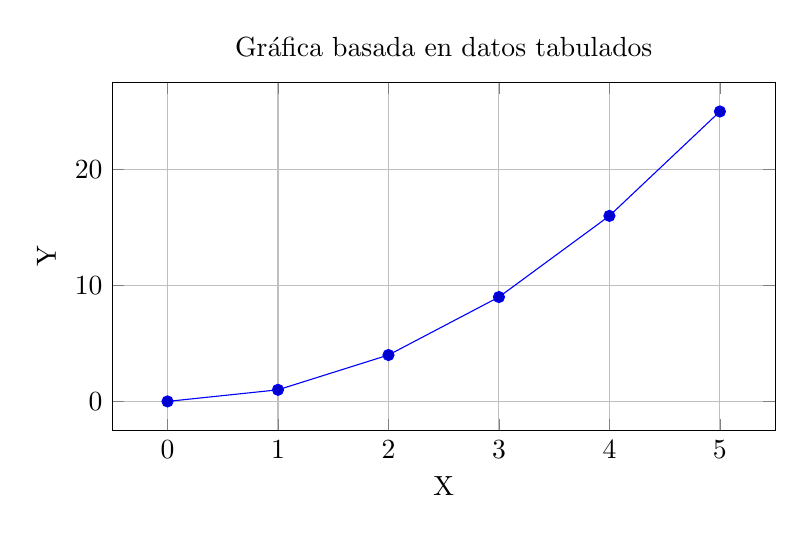
\begin{tikzpicture}
        \begin{axis}[
            title={Gráfica basada en datos tabulados},
            xlabel={X},
            ylabel={Y},
            grid=major, % Añade una cuadrícula mayor
            width=10cm, % Ancho de la gráfica
            height=6cm, % Altura de la gráfica
        ]
        % Datos tabulados para la gráfica
        \addplot table[row sep=\\, y index=1] {
            x y  \\
            0 0  \\
            1 1  \\
            2 4  \\
            3 9  \\
            4 16 \\
            5 25 \\
        };
        \end{axis}
    \end{tikzpicture}
    \caption{Ejemplo de gráfica creada a partir de una tabla de datos}
    \label{fig:tabla_grafica}
\end{figure}
\textbf{\large{\href{https://youtu.be/dQw4w9WgXcQ?si=jGf-LdN459y-xefY}{EJEMPLO DE URL (LINK)}}}
\end{document}